\documentclass{article}
\usepackage{amsmath, amsfonts, graphicx, hyperref, xcolor, indentfirst, float}
\usepackage[utf8]{inputenc}
\usepackage[italian]{babel}
\linespread{1.2}
\hypersetup{
    colorlinks=false,
    linkbordercolor=white
}
\setlength{\parindent}{0pt}


\begin{document}


\numberwithin{equation}{subsection}
\title{Oscillatore armonico su reticolo}
\author{Lorenzo Tasca}
\date{Gennaio 2024}
\maketitle


\tableofcontents
\newpage
\section{Introduzione}
In questo lavoro illustriamo come affrontare lo studio di un sistema quantistico in maniera non perturbativa mediante l'impiego di tecniche numeriche Montecarlo per il calcolo del path integral. È ben noto infatti che molti sistemi quantistici complessi non sono risolvibili in modo esatto, rendendo indispensabile l'utilizzo di approcci approssimati. Una strada è rappresentata dall'approccio perturbativo, che consiste nell'effettuare uno sviluppo nella costante di accoppiamento del sistema, tuttavia esistono molti fenomeni che non sono trattabili in questo modo. Il path integral permette di poter analizzare il sistema in maniera totalmente non perturbativa. \\Ci concentreremo sul caso di un potenziale armonico monodimensionale, in quanto essendo un sistema semplice è possibile confrontare il nostro risultato con quello esatto. Tuttavia i metodi illustrati sono del tutto generali e posso essere facilmente utilizzati con un potenziale generico e, con i dovuti adattamenti, anche nelle teorie quantistiche di campo. \\
L'idea fondamentale di questa tecnica consiste nel fatto che discretizzando il tempo il path integral si riduce ad un integrale in un numero finito di dimensioni, e può pertanto essere calcolato tramite tecniche Montecarlo. Come illustreremo è poi possibile legare tale integrale a diverse grandezze significative del sistema, come le differenze tra i livelli energetici o gli elementi di matrice. Una volta calcolato l'integrale è quindi possibile risalire a tali grandezze di importanza fisica. Nel nostro caso, a titolo di esempio, calcoleremo la differenza di energia $E_1-E_0$ tra i primi due autostati del sistema, e l'elemento di matrice $\left<1|\hat{x}|0\right>$.






\section{Preliminari teorici}

 Come anticipato lavoreremo con un oscillatore armonico quantistico monodimensionale, ossia un sistema la cui Lagrangiana nel continuo è data da \footnote{Da qui in avanti lavoreremo sempre usando il tempo euclideo e $\hbar=1$.}
\begin{equation}
    \mathcal{L}=\frac{1}{2}m\dot{x}^2+\frac{1}{2}m\omega^2x^2.
\end{equation}
Tale sistema può essere risolto esattamente, risolvendo analiticamente l'equazione di Schrödinger stazionaria, ed è ben noto che presenta infiniti stati legati non degeneri $\left|n\right>$ con energia 
\begin{equation}
    E_n=\omega\left(n+\frac{1}{2}\right).
\end{equation}

\subsection{Trattazione con path integral}


Lo studio di un sistema quantistico può essere formulato in maniera del tutto equivalente a quella tradizionale utilizzando il path integral. In tale formalismo il tempo viene discretizzato in un reticolo di passo reticolare $a$, composto da $N$ siti reticolari, utilizzando condizioni al bordo periodiche. Possiamo senza perdita di generalità partire da $t=0$ e definire $T=N\cdot a$, avremo quindi 
\begin{equation}
    t_i=a\cdot i, \,\,\,\,\,\, i=0,\cdots, N-1, 
\end{equation}
con 
\begin{equation}
    x(T)=x(0).
\end{equation}
\subsubsection{Funzioni di correlazione}
Le grandezze fondamentali calcolabili mediante il path integral sono le funzioni di correlazione, poiché, come vedremo, sono direttamente legate alle osservabili fisiche.  In particolare date due osservabili generiche $O_1(x)$ e $O_2(x)$ si definisce la funzione di correlazione a due punti come 
\begin{equation}
    \label{stufa}
    c\,(t_1=i_1a, t_2=i_2a)=\int \prod_{i=0}^{N-1} dx_i\,O_1(x_{i_1})O_2(x_{i_2})\frac{e^{-S}}{Z}, 
\end{equation}
dove 
\begin{equation}
    \label{azione}
    S=a\sum_{i=0}^{N-1} \mathcal{L}(x_{i+1}, x_i)=a\sum_{i=0}^{N-1} \frac{1}{2}m\left(\frac{x_{i+1}-x_i}{a}\right)^2+\frac{1}{2}m\omega^2x_i^2,
\end{equation}
è l'azione discretizzata su reticolo, mentre 
\begin{equation}
    Z=\int \prod_{i=0}^{N-1} dx_i\, e^{-S},
\end{equation}
è la funzione di partizione del sistema. \\
Sottolineiamo sin da subito che l'integrale in (\ref{stufa}) dal punto di vista formale risulta essere un ordinario integrale in $N$ dimensioni, e può essere quindi approcciato mediante opportune tecniche numeriche. Tali tecniche calcoleranno il correlatore in modo approssimato, ma è importante notare che non è stato fatto alcun sviluppo nella costante di accoppiamento. 

\subsubsection{Matrice di trasferimento}

Si definisce la matrice di trasferimento $\hat{T}_a$ come 
\begin{equation}
    \hat{T_a}=\exp{\left(-\frac{1}{2}aV(\hat{x})\right)}\exp{\left(-a\frac{\hat{p}^2}{2m}\right)}\exp{\left(-\frac{1}{2}aV(\hat{x})\right)},
\end{equation}
dove nel nostro caso $V(\hat{x})=\frac{1}{2}m\omega^2\hat{x}^2$.\\
Siccome $\hat{T}_a$ è un'operatore unitario è possibile scriverlo nella forma 
\begin{equation}
    \hat{T_a}=\exp{\left(-a\hat{\bar{H}}\right)},
\end{equation}
dove $\hat{\bar{H}}$ è un operatore autoaggiunto. \\Definiamo gli autostati $\left|\varepsilon_n\right>$ dell'operatore $\hat{\bar{H}}$
\begin{equation}
    \hat{\bar{H}}\left|\varepsilon_n\right>=\varepsilon_n\left|\varepsilon_n\right>,
\end{equation}
\begin{equation}
    \label{miaomiao}
    \hat{T_a}\left|\varepsilon_n\right>=e^{-a\varepsilon_n}\left|\varepsilon_n\right>.
\end{equation} 
Poiché $\hat{\bar{H}}$ è un operatore autoaggiunto essi formano una base completa dello spazio di Hilbert. Espandendo l'esponenziale, si può osservare che l'operatore di evoluzione temporale può essere espresso come
\begin{equation}
    \exp{\left(-a\hat{H}\right)}=\exp{\left(-a\hat{\bar{H}}\right)}+o(a),
\end{equation}
e che conseguentemente
\begin{equation}
    \label{eps=E+o(a)}
    \varepsilon_n=E_n+o(a),
\end{equation}
quindi $\hat{T}_a$ propaga uno stato generico di uno step temporale $a$, a meno di errori di discretizzazione.\\
Si può mostrare che le funzioni di correlazione si possono scrivere come (assumendo senza perdità di generalità che $t_2>t_1$)
\begin{equation}
    \label{c_con_T}
    c\,(t_1,t_2)=\frac{1}{Z} \textup{Tr}\left[\hat{T}_a^{N-i_2-i_1}\,\hat{O}_2\,\hat{T}^{i_2-i_1}\,\hat{O}_1\right], 
\end{equation}
e conseguentemente $Z$ risulta essere
\begin{equation}
    \label{Z con T^N}
    Z=\textup{Tr}\left[\hat{T_a}^N\right].
\end{equation}




\subsection{Estrarre informazioni dai correlatori}
 
Illustreremo ora come, a partire dalla funzione di correlazione a due punti (calcolabile numericamente), è possibile estrarre le due quantità fisiche che ci interessa valutare, ovvero la differenza di energia $\Delta E$ tra lo stato $\left|0\right>$ e lo stato $\left|1\right>$, e l'elemento di matrice $\left<1|\hat{x}|0\right>$.\\
Esplicitiamo la traccia nella (\ref{Z con T^N}) sommando sugli autostati di $\hat{\bar{H}}$, usando la (\ref{miaomiao}) otteniamo così 
\begin{equation}
    Z=\sum_n \left<\varepsilon_n\right|\hat{T}_a^N\left|\varepsilon_n\right>=\sum_n e^{-aN\varepsilon_n}.
\end{equation}
Analogamente prendendo la traccia nella (\ref{c_con_T}) abbiamo \footnote{Ricordiamo sempre che abbiamo posto $t_2>t_1$ per semplicità di scrittura della formula.}
\begin{equation}
    c\,(t_1,t_2)=\frac{1}{Z} \sum_n e^{-\varepsilon_n(T-t_2-t_1)}\left<\varepsilon_n\right|\hat{O}_2\,\hat{T}^{i_2-i_1}\,\hat{O}_1\left|\varepsilon_n\right>.
\end{equation}
Inseriamo un'identità  $\sum_m \left|\varepsilon_m\right>\left<\varepsilon_m\right|$ adiacente alla matrice di trasferimento e usiamo ancora la (\ref{miaomiao}):

\begin{equation}
    c\,(t_1, t_2)=\frac{1}{Z}\sum_{n,m} e^{-\varepsilon_n(T-t_2-t_1)}e^{-\varepsilon_m(t_2-t_1)}\left<\varepsilon_n\right|\hat{O}_2\left|\varepsilon_m\right>\left<\varepsilon_m\right|\hat{O}_1\left|\varepsilon_n\right>.
\end{equation}
Andiamo ora a scegliere $\hat{O}_1=\hat{O}_2=\hat{x}$ e prendiamo anche i limiti $N\rightarrow+\infty$ e $t_2-t_1\rightarrow+\infty$ per estrarre l'esponenziale dominante nelle somme. L'esponenziale dominante in $Z$ è $e^{-\varepsilon_0T}$, mentre quello a numeratore è quello con $m=n=0$, ma l'elemento di matrice $\left<\varepsilon_0\right|\hat{x}\left|\varepsilon_0\right>$ è nullo in un oscillatore armonico, pertanto il primo termine non nullo che sopravvive nella somma è quello con $n=1$ ed $m=0$ e quello con $n=0$ ed $m=1$. Conseguentemente abbiamo 
\begin{equation}
    c\,(t_1,t_2)=\frac{e^{-(N-i_2-i_1)a\varepsilon_0}e^{-(i_2-i_1)a\varepsilon_1}+e^{-(N-i_2-i_1)a\varepsilon_1}e^{-(i_2-i_1)a\varepsilon_0}}{e^{-a\varepsilon_0N}}\left|\left<\varepsilon_0\right|\hat{x}\left|\varepsilon_1\right>\right|^2,
\end{equation}
 che può essere riscritta come 
 \begin{equation}
    c(t_1,t_2)=2\left|\left<\varepsilon_0\right|\hat{x}\left|\varepsilon_1\right>\right|^2e^{-\frac{N}{2}a(\varepsilon_1-\varepsilon_0)}\cosh\left(\left(\frac{N}{2}-(i_2-i_1)\right)a(\varepsilon_1-\varepsilon_0)\right).
 \end{equation}
Per via delle condizioni al bordo periodiche tale correlatore non dipenderà direttamente dai valori di $t_1$ e $t_2$, ma solo dalla loro differenza. Possiamo quindi chiamare $t=t_2-t_1$ e $i=\frac{t}{a}$, ottenendo così
\begin{equation}
    \label{ho fame}
    c(t)=2\left|\left<\varepsilon_0\right|\hat{x}\left|\varepsilon_1\right>\right|^2e^{-\frac{N}{2}a(\varepsilon_1-\varepsilon_0)}\cosh\left(\left(\frac{N}{2}-i\right)a(\varepsilon_1-\varepsilon_0)\right).
\end{equation}
A partire dal correlatore $c(t)$ è possibile estrarre la differenza di energia $\Delta\varepsilon=\varepsilon_1-\varepsilon_0$ prendendo
\begin{equation}
    \label{nuvola}
    \Delta\varepsilon=\frac{1}{a}\cosh^{-1}\left(\frac{c(t+1)+c(t-1)}{2c(t)}\right).
\end{equation}
Infatti 
$$\frac{c(t+1)+c(t-1)}{2c(t)}=\frac{\cosh\left[\left(\frac{T}{2}-t-a\right)\Delta\varepsilon\right]+\cosh\left[\left(\frac{T}{2}-t+a\right)\Delta\varepsilon\right]}{2\cosh\left[\left(\frac{T}{2}-t\right)\Delta\varepsilon\right]}=\cosh(a\Delta\varepsilon),$$
dove abbiamo usato che $\cosh(x)+\cosh(y)=2\cosh\left(\frac{x+y}{2}\right)\cosh\left(\frac{x-y}{2}\right).$\\
Una volta trovato $\Delta\varepsilon$ possiamo trovare l'elemento di matrice a partire dalla (\ref{ho fame}). Per semplicità possiamo assumere di lavorare nel regime in cui $\frac{N}{2}$ è grande rispetto a $t$ e usare che $\cosh x\approx \frac{e^x}{2}$ in tale regime, ottenendo così 
\begin{equation}
    \label{bea}
    \left|\left<\varepsilon_0\right|\hat{x}\left|\varepsilon_1\right>\right|=\sqrt{c(t)\exp{\left(ta\Delta\varepsilon\right)}}.
\end{equation}
Siamo pertanto riusciti a ridurre il calcolo delle due quantità fisiche a cui siamo interessati al calcolo del correlatore 
\begin{equation}
    \label{correlatore}
    c\,(t)=\int \prod_{i=0}^{N-1} dx_i\, x_hx_{i+h}\,\frac{e^{-S}}{Z},
\end{equation}
dove $t=ia$, e il correlatore non dipenderà dal valore di $h$ per via delle condizioni al bordo periodiche. Una volta noto quest'ultimo possiamo facilmente trovare $\Delta\varepsilon$ e $\left|\left<\varepsilon_0\right|\hat{x}\left|\varepsilon_1\right>\right|$ usando la (\ref{nuvola}) e la (\ref{bea}). Dopo aver ottenuto le grandezze su reticolo, sarà necessario prendere il limite $a\rightarrow 0$ per estrarre le quantità nel continuo:
\begin{equation}
    \lim_{a\rightarrow0}\Delta\varepsilon=E_1-E_0,
\end{equation}
\begin{equation}
    \lim_{a\rightarrow0}\left|\left<\varepsilon_0\right|\hat{x}\left|\varepsilon_1\right>\right|=\left|\left<0\right|\hat{x}\left|1\right>\right|.
\end{equation}
Altre scelte degli operatori $\hat{O}_1$ e $\hat{O}_2$ (oppure considerare funzioni di correlazione di ordine più alto) danno la possibilità di estrarre altre quantità fisiche.








\subsection{Metodo Montecarlo per valutare il path integral}

Al fine di calcolare numericamente $c\,(t)$ è necessario valutare il path integral in (\ref{correlatore}). Si tratta di un integrale multidimensionale in $N$ variabili reali, con $N$ grande, pertanto al fine di valutare l'integrale è necessario ricorrere a tecniche probabilistiche Montecarlo, in quanto le tecniche deterministiche di calcolo dell'integrale sono efficienti soltanto se $N<10$.\\ Supponiamo in tutta generalità di voler valutare un integrale della forma 
\begin{equation}
    I=\int \prod_{i=0}^{N-1} dx_i\, {f(x_0,\cdots, x_{N-1})}{g(x_0,\cdots, x_{N-1})},
\end{equation}
e supponiamo di avere $M$ set di variabili aleatorie $(x_0^k,\cdots, x_{N-1}^k)_{k\in\{1,\cdots,M\}}$, ciascun set con distribuzione di probabilità $g(x_0,\cdots, x_{N-1})$. Allora la variabile aleatoria 
\begin{equation}
    \hat{I}=\frac{1}{M}\sum_{k=1}^{M}f(x_0^k,\cdots,x_{N-1}^k),
\end{equation}
è tale che 
\begin{equation}
    \mathbb{E}(\hat{I})=I.
\end{equation}
Infatti chiamando $y^k=f(x_0^k,\cdots,x_{N-1}^k)$ si ha che 
$$\mathbb{E}(y^k)=\int d{y^k}\, p(y^k){y^k}=$$$$=\int dy^k\prod_i dx_i\, \delta\left(y^k-f(x_0^k,\cdots,x_{N-1}^k)\right)p(x_0,\cdots, x_{N-1})y^k=$$$$=\int \prod_i dx_i\, {g(x_0,\cdots, x_{N-1})}{f(x_0,\cdots, x_{N-1})}=I,$$
e conseguentemente 
\begin{equation}
    \mathbb{E}(\hat{I})=\frac{1}{M}\sum_{k=1}^{M}\mathbb{E}[f(x_0^k,\cdots,x_{N-1}^k)]=I.
\end{equation}
Nel nostro caso (eq. (\ref{correlatore})) avremo che 
\begin{equation}
    f(x_0,\cdots, x_{N-1})=x_{h}x_{h+t/a},
\end{equation}
\begin{equation}
    g(x_0,\cdots, x_{N-1})=\frac{e^{-S}}{Z},
\end{equation}
pertanto date $M$ configurazioni $(x_0^k,\cdots, x_{N-1}^k)_{k\in\{1,\cdots,M\}}$ estratte con probabilità $\frac{e^{-S}}{Z}$ abbiamo che 
\begin{equation}
    c\,(t)\simeq\frac{1}{M}\sum_{k=1}^{M} x_{h}^kx_{h+t/a}^k.
\end{equation}
In questo caso specifico, siccome $c\,(t)$ non dipende dal valore di $h$, possiamo anche mediare sui valori di $h$, ridefinendo $c\,(t)$ come 
\begin{equation}
    c\,(t)=\frac{1}{M}\frac{1}{N}\sum_{k=1}^{M}\sum_{h=0}^{N-1} x_{h}^kx_{h+t/a}^k=\sum_{k=1}^{M}c^k(t),
\end{equation}
dove abbiamo definito 
\begin{equation}
    \label{vasca da bagno}
    c^k(t)=\frac{1}{N}\sum_{h=0}^{N-1} x_{h}^kx_{h+t/a}^k.
\end{equation}
Abbiamo quindi ridotto il calcolo del correlatore al calcolo di una somma, a patto di essere in grado di generare le configurazioni con probabilità $\frac{e^{-S}}{Z}$.
Per fare ciò utilizzeremo l'algoritmo del Metropolis, che andremo ora a richiamare. 







\subsection{Algoritmo del Metropolis}
Supponiamo di voler generare numeri con probabilità $g(x_0,\cdots, x_{N-1})$.
L'algoritmo prevede che, a ogni step (chiamati \textit{sweep}), per ogni variabile di integrazione $x_i$ venga proposto un nuovo valore $x_i'$ distribuito uniformemente in $[x_i-\Delta, x_i+\Delta]$, dove $\Delta$ è un numero reale scelto in maniera arbitraria. Si calcola poi la quantità 
\begin{equation}
    r=\frac{g(x_0, \cdots, x'_i, \cdots, x_{N-1})}{g(x_0, \cdots, x_i, \cdots, x_{N-1})},
\end{equation}
e il valore proposto viene poi accettato secondo la seguente prescrizione:
\begin{itemize}
    \item se $r>1$ viene accettato con probabilità 1,
    \item se $r<1$ viene accettato con probabilità $r$.
\end{itemize}
Se il valore non viene accettato allora il valore di $x_i$ non viene modificato nello sweep. Tale prescrizione permette di arrivare a generare numeri distribuiti secondo $g$ a partire da qualsiasi configurazione iniziale $(x_0^{in},\cdots,x_{N-1}^{in})$, dopo un certo numero di sweep di termalizzazione (che andranno stimati).
Nel nostro caso specifico abbiamo che 
\begin{equation}
    \label{r metropolis}
    r=e^{-\Delta S},
\end{equation}
con 
\begin{equation}
    \Delta S=S(x_0, \cdots, x'_i, \cdots, x_{N-1})-S(x_0, \cdots, x_i, \cdots, x_{N-1}).
\end{equation}
Siccome l'algoritmo del Metropolis può essere pensato come una catena di Markov, spesso ci si riferisce all'indice dello sweep come \textit{tempo markoviano}. \\ La scelta di $\Delta$ è arbitraria, nel senso che ogni valore darà in media gli stessi risultati, tuttavia influenza altri fattori come la durata della simulazione e la correlazione tra due configurazioni successive (che discuteremo in seguito). Pertanto è importante scegliere un valore di $\Delta$ opportuno per poter simulare il sistema in modo efficace. In particolare possiamo definire l'accettanza di uno sweep come 
\begin{equation}
    \label{accettanza}
    \textup{accettanza}=\frac{\textup{numero di variabili di integrazione modificate}}{N}.
\end{equation}
È consigliabile scegliere $\Delta$ in modo che l'accettanza media sia compresa tra $50\%$ e $80\%$. 



\subsection{Correlazione tra le configurazioni}

Il valore atteso della variabile aleatoria $\hat{I}$ coincide con il path integral che vogliamo calcolare, ma è necessario studiarne anche la varianza al fine di associare un errore a $c\,(t)$ e di conseguenza alle quantità fisiche che ne derivano. \\ Se le varie configurazioni estratte dal Metropolis fossero indipendenti, allora sapremmo facilmente valutare la varianza utilizzando il teorema del limite centrale, però non è questo il caso. Nel nostro caso abbiamo che 
\begin{equation}
    c\,(t)\simeq \frac{1}{M}\sum_{k=1}^{M}c^k(t)
\end{equation}
dove $k$ è un indice di tempo markoviano, $M$ è il numero totale di sweep e $c^k(t)$ è definito dalla (\ref{vasca da bagno}). È possibile mostrare che 
\begin{equation}
    \sigma^2(c(t))=\frac{\sigma^2(c^k(t))}{M}\left[1+2\sum_{t_M=1}^{+\infty}\frac{\Gamma(t,t_M)}{\Gamma(t,0)}\right],
\end{equation}
dove 
\begin{equation}
    \label{equazione gamma}
    \Gamma(t, t_M)=\mathbb{E}[c^k(t)c^{k+t_M}(t)]-\left(\mathbb{E}[c^k(t)]\right)^2.
\end{equation}
Se le variabili $c^k(t)$ fossero scorrelate a $k$ diverse, allora $\Gamma=0$ e ritroveremmo la classica formula fornita del teorema del limite centrale. Avere $\Gamma\neq0$ quindi va a quantificare quanto la variabili sono correlate a una distanza markoviana pari a $t_M$. Si definisce \textit{tempo di decorrelazione} $\tau$ il valore minimo di $t_M$ per cui $\Gamma$ risulta essere sostanzialmente nulla. 
\begin{equation}
    \Gamma(t,\tau)\simeq 0.
\end{equation}
Tale tempo può essere stimato nelle simulazioni. Se decidiamo però di voler lavorare con variabili non correlate tra di loro nel tempo markoviano abbiamo due possibilità:
\begin{itemize}
    \item saltare un numero di sweep pari a $\tau$, ovvero calcolare $c^k(t)$ solo se $k$ è multiplo di $\tau$. Questa scelta è da intraprendere nel caso in cui calcolare $c^k(t)$ sia più costoso che far evolvere il Metropolis per $\tau$ sweep;
    \item suddividere le configurazioni in bin di grandezza $D_{\textup{BIN}}=\tau$ e mediare $c^k(t)$ all'interno di ogni bin. Nel nostro caso questa è la scelta migliore, in quanto calcolare l'osservabile è poco costoso e effettuare la media ci permette di non far evolvere il Metropolis a vuoto. Avremo un numero di bin $N_{\textup{BIN}}$ tale che $N_{\textup{BIN}}\cdot D_{\textup{BIN}}=M$.
\end{itemize}
Definiamo quindi 
\begin{equation}
    \label{cbinnate}
    c^k_{\textup{BIN}}(t)=\frac{1}{D_{\textup{BIN}}}\sum_{j=0}^{D_{\textup{BIN}}-1} c^{k+j}(t),
\end{equation}
mediando all'interno del bin. Per quanto discusso $c^k_{\textup{BIN}}(t)$ non è correlato con $c^{k+1}_{\textup{BIN}}(t)$. Il correlatore $c(t)$ si calcola ora come 
\begin{equation}
    \label{che freddo}
    c\,(t)\simeq \frac{1}{N_{\textup{BIN}}} \sum_{k=0}^{N_{\textup{BIN}-1}} c_{\textup{BIN}}^k(t),
\end{equation}
dove i vari addendi nella somma sono tra loro scorrelati.


\subsection{Propagazione degli errori}

Una volta calcolato il correlatore con la (\ref{che freddo}), possiamo andare a calcolare la differenza di energia $\Delta \varepsilon$ e l'elemento di matrice. È necessario però capire come propagare l'errore per ottenere una stima dell'errore sulle quantità finali. Per fare ciò useremo il formalismo del Jackknife. Consideriamo le $N$ variabili aleatorie $c_{\textup{BIN}}(t)$ indicizzate dall'indice di tempo fisico $t$. Tali variabili verranno chiamate primarie. Abbiamo visto che possiamo estrarre $N_{\textup{BIN}}$ campionamenti \textit{indipendenti} delle variabili primarie $\{c_{\textup{BIN}}^k(t)\}_{k\in \{0,\cdots, N_{\textup{BIN}}-1\}}$. Il correlatore si calcola poi come il valor medio di questi campionamenti
\begin{equation}
    c\,(t)=\frac{1}{N_{\textup{BIN}}}\sum_{k=0}^{N_{\textup{BIN}}-1} c_{\textup{BIN}}^k(t).
\end{equation}
Definiamo i cluster Jackknife delle variabili primarie come 
\begin{equation}
    \textup{cluster}_c^k(t)=c\,(t)-\frac{c^k(t)-c(t)}{N-1}.
\end{equation}
Supponiamo di considerare poi la variabile aleatoria (secondaria)
\begin{equation}
    F=f(c\,(t=0), \cdots, c\,(t=N-1)),
\end{equation}
dove la particolare forma della funzione $f$ dipenderà da quale quantità fisica vogliamo calcolare, secondo le equazioni (\ref{nuvola}) e (\ref{bea}). 
L'asserto del Jackknife è che la variabile aleatoria
\begin{equation}
    \label{che fame}
    \sigma^2_{\mathrm{JACK}}({F})=\frac{N_{\textup{BIN}}-1}{N_{\textup{BIN}}}\sum_{k=0}^{N_{\textup{BIN}}-1}\left(\textup{cluster}^k_F-{F}\right)^2,
\end{equation}
è uno stimatore della varianza di $F$, dove i cluster di $F$ sono definiti come 
\begin{equation}
    \textup{cluster}^k_F=f(\textup{cluster}_c^k(t=0), \cdots, \textup{cluster}_c^k(t=N-1)).
\end{equation}
Tale asserto può essere verificato a partire dal fatto che 
$$\textup{cluster}^k_F=f(\textup{cluster}_c^k(t_i))
=f\left(c\,(t_i)-\frac{c^k(t_i)-c(t_i)}{N_{\textup{BIN}}-1}\right)=$$
$$=F-\sum_{i=0}^{N-1}\frac{\partial f}{\partial c(t_i)}\frac{\textup{cluster}_c^k(_i)-c(t_i)}{N_{\textup{BIN}}-1}+o\left(\frac{1}{N_{\textup{BIN}}}\right), $$
che inserita nella (\ref{che fame}) fornisce la classica formula di propagazione degli errori. \\
Rimarchiamo che la tecnica del Jackknife è utilizzabile solo nel caso di campionamenti \textit{indipendenti} della variabili primarie, quindi è cruciale generare le $c_{\textup{BIN}}^k(t)$ senza correlazione, effettuando il binnaggio dopo aver stimato il tempo di autocorrelazione.



\subsection{Soluzione esatta su reticolo}

L'oscillatore armonico possiede una soluzione esatta anche su reticolo, ovvero è possibile diagonalizzare esattamente la matrice di trasferimento $\hat{T}_a$ e quindi estrarre i suoi autostati $\left|\varepsilon_n\right>$ e i suoi autovalori $e^{-a\varepsilon_n}$. Questo ci permette di confrontare il risultato della simulazione con il valore atteso teorico anche a passo reticolare finito, quindi prima di prendere il limite al continuo. \\
In particolare si può dimostrare che l'Hamiltoniana efficace
\begin{equation}
    \hat{H}_{\textup{eff}}=\frac{\hat{p}^2}{2m}+\frac{1}{2}m\omega_{\textup{eff}}^2\hat{x}^2,
\end{equation}
con 
\begin{equation}
    \omega_\textup{eff}=\omega\sqrt{1+\frac{a^2\omega^2}{4}},
\end{equation}
commuta con la matrice di trasferimento, quindi risulta essere diagonale nella base $\left|\varepsilon_n\right>$, da cui consegue che, come per l'oscillatore armonico tradizionale,
\begin{equation}
    \label{el mat esatto}
    \left<\varepsilon_0\right|\hat{x}\left|\varepsilon_1\right>=\frac{1}{\sqrt{2m\omega_\textup{eff}}}.
\end{equation}
Inoltre vale che 
\begin{equation}
    \label{energia esatto}
    \varepsilon_n=\frac{1}{a}\left(n+\frac{1}{2}\right)\log\left(a\omega_\textup{eff}+1+\frac{a^2\omega^2}{2}\right).
\end{equation}

\subsection{Errore relativo}

Le equazioni (\ref{nuvola}) e (\ref{bea}) ci dicono che ogni valore di $t$ utilizzato per calcolare il correlatore $c\,(t)$ di principio dovrebbe restituire lo stesso risultato fisico, ovvero lo stesso gap energetico e lo stesso elemento di matrice. Il valore numerico stimato avrà però delle fluttuazione casuali, è quindi ragionevole mediare sui vari valori di $t$ e calcolare le osservabili come 
\begin{equation}
    \label{panca piana}
    \Delta\varepsilon=\frac{1}{N}\sum_{t=0}^{N-1}\frac{1}{a}\cosh^{-1}\left(\frac{c(t+1)+c(t-1)}{2c(t)}\right),
\end{equation} 
\begin{equation}
    \label{panca inclinata}
    \left|\left<\varepsilon_0\left|\hat{x}\right|\varepsilon_1\right>\right|=\frac{1}{N}\sum_{t=0}^{N-1}\sqrt{c(t)\exp{\left(ta\Delta\varepsilon\right)}},
\end{equation}
o ancora meglio potremmo effettuare una media pesata sull'errore. 
Se andiamo però a vedere l'errore relativo di $c\,(t)$ al variare di $t$ ci accorgiamo che non tutti i valori di $t$ possono essere utilizzati per effettuare tale media, in quanto alcuni hanno un errore relativo molto grosso e sono pertanto sostanzialmente rumore. L'errore relativo per definizione si calcola come
\begin{equation}
    \frac{\sigma^2(c(t))}{c(t)^2}=\frac{1}{N_{\textup{sweep}}}\left[\frac{c_{x^2x^2}(t)}{c(t)^2}-1\right], 
\end{equation} 
dove $c_{x^2x^2}(t)$ è il correlatore
\begin{equation}
    c_{x^2x^2}(t)=\int \prod_{i=0}^{N-1} dx_i\,x_{h}^2x_{h+t}^2\,\frac{e^{-S}}{Z}.
\end{equation}
Quest'ultimo si può calcolare a partire dalla (\ref{c_con_T}) analogamente a come illustrato per $c\,(t)$, e nel limite in cui $N$, $t$ e $\frac{N}{2}-t$ sono grandi, usando anche la (\ref{ho fame}) otteniamo che 
\begin{equation}
    \frac{\sigma^2(c(t))}{c(t)^2}=\frac{1}{N_{\textup{sweep}}}\frac{  \left|\left<\varepsilon_0\right|\hat{x}^2\left|\varepsilon_0\right>\right|}{  \left|\left<\varepsilon_0\right|\hat{x}\left|\varepsilon_1\right>\right|}\exp\left(2t(\varepsilon_1-\varepsilon_0)\right).
\end{equation}
Conseguentemente al crescere di $t$ l'errore relativo cresce esponenzialmente, rendendo pertanto inutilizzabili i risultati calcolati per tali valori di $t$. Si può quindi ad esempio scegliere di effettuare la media solo per i valori di $t$ per cui l'errore relativo è inferiore al 10\%. 


























\newpage
\section{Risultati della simulazione}

\subsection{Panoramica}
I punti discussi possono essere implementati in un calcolatore per effettuare il calcolo completo ed ottenere una stima per le osservabili fisiche considerate. Riassumiamo qui i punti principali della simulazione. \\ Il punto fondamentale è il calcolo del correlatore $c\,(t)$, che secondo la 
(\ref{che freddo}) si calcola come 
\begin{equation}
    c\,(t)= \frac{1}{N_{\textup{BIN}}} \sum_{k=0}^{N_{\textup{BIN}-1}} c_{\textup{BIN}}^k(t),
\end{equation}
ove 
\begin{equation}
    \label{guido}
    c^k_{\textup{BIN}}(t)=\frac{1}{D_{\textup{BIN}}}\sum_{j=0}^{D_{\textup{BIN}}-1} \frac{1}{N}\sum_{h=0}^{N-1} x_{h}^{k+j}x_{h+t/a}^{k+j},
\end{equation}
con le configurazioni $(x_0^k,\cdots, x_{N-1}^k)$ generate con il Metropolis con probabilità $\frac{e^{-S}}{Z}$. È necessario quindi implementare:
\begin{itemize}
    \item calcolo del tempo di termalizzazione, per stabilire dopo quanti sweep si generano numeri con la probabilità voluta $\frac{e^{-S}}{Z}$;
    \item calcolo del tempo di autocorrelazione, per stabilire la grandezza dei bin da utilizzare nella (\ref{guido});
    \item calcolo effettivo del correlatore tramite la somma in (\ref{guido}).
\end{itemize}
Dopo aver ottenuto il valore del correlatore possiamo ottenere i valori fisici a cui siamo interessati usando le equazioni (\ref{nuvola}) e (\ref{bea}), propagando l'errore utilizzando la tecnica del Jackknife, per poi effettuare una media sui valori di $t$ come discusso nella (\ref{panca piana}) e (\ref{panca inclinata}). \\ Sarà necessario poi prendere il limite $a\rightarrow 0$ per ottenere il valore nel continuo. 







\subsection{Scelta dei parametri}

Nel calcolatore abbiamo memorizzato i parametri fisici per unità di passo reticolare, quindi al fine di prendere il limite al continuo bisognerà agire su questi. In particolare l'azione in (\ref{azione}) si scrive come 
\begin{equation}
    S=\sum_{i=0}^{N-1} \frac{1}{2}M\left(x_{i+1}-x_i\right)^2+\frac{1}{2}M\Omega^2x_i^2,
\end{equation}
dove 
\begin{equation}
    M=\frac{m}{a},
\end{equation}
\begin{equation}
    \Omega=a\omega,
\end{equation}
sono la massa e la frequenza per unità di passo reticolare. Inoltre abbiamo che l'intervallo totale di tempo in cui lavoriamo è 
\begin{equation}
    T=aN.
\end{equation}
Modificare $M$, $\Omega$ ed $N$ (che sono memorizzati nel calcolatore) equivale a modificare $a$, se pensiamo di mantenere i parametri fisici $m$, $\omega$ e $T$ fissati. In particolare scegliamo di usare $\omega=1$ e $m=1$. I valori usati per le simulazioni sono riportati in Tabella \ref{tabella vari reticoli}.
\begin{table}[h]
    \centering
    \begin{tabular}{||c c c c||} 
     \hline
     $N$ & $M$ & $\Omega$ & $a$ \\ [0.5ex] 
     \hline\hline
     32 & 0.5 & 2 & 2 \\ 
     64 & 1 & 1 & 1 \\
     128 & 2 & 0.5 & 0.5 \\
     256 & 4 & 0.25 & 0.25 \\ 
     512 & 8 & 0.125 & 0.125 \\ 
     1024 & 16 & 0.0625 & 0.0625 \\ [1ex] 
     \hline
    \end{tabular}
    \caption{Valori dei parametri nel calcolatore nelle varie simulazioni.}
    \label{tabella vari reticoli}
\end{table}\\
Effettueremo quindi la simulazione per ogni set di parametri, per poi effettuare una estrapolazione ad $a=0$. 

\subsection{Scelta di $\Delta$ e accettanza}
L'algoritmo del Metropolis propone dei numeri uniformemente con ampiezza $\Delta$, che verranno poi accettati o rigettati. $\Delta$ non influenza la correttezza della simulazione, ma va scelto un valore che renda il calcolo più efficiente possibile. L'accettanza del Metropolis definita nella (\ref{accettanza}) dipende dal parametro $\Delta$, oltre che dal passo reticolare. Rappresentiamo in Figura \ref{grafico accettanza} l'accettanza media calcolata per $N=64$, al variare del parametro $\Delta$.
\begin{figure}[h]
    \centering
    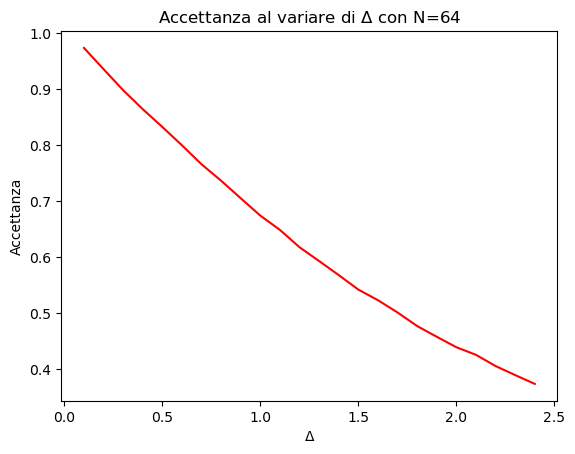
\includegraphics[width=0.7\textwidth]{images/accettanza_N64.png}
    \caption{Accettanza media al variare di $\Delta$ per $N=64$}
    \label{grafico accettanza}
\end{figure}

Possiamo scegliere $\Delta=1$ in modo da ottenere un'accettanza adeguata. 
L'accettanza per $\Delta=1$ ottenuta per i diversi passi reticolari è riportata in Tabella \ref{tabella accettanza}. 
\begin{table}[h]
    \centering
    \begin{tabular}{||c c||} 
     \hline
     $N$ & Accettanza  \\ [0.5ex] 
     \hline\hline
     32 & 68\% \\ 
     64 & 67\%  \\
     128 & 62\%  \\
     256 & 51\%  \\ 
     512 & 39\%  \\
     1024 & 28\%  \\[1ex] 
     \hline
    \end{tabular}
    \caption{Accettanza media con $\Delta=1$ al variare di $N$}
    \label{tabella accettanza}
\end{table}

L'andamento in Figura \ref{grafico accettanza} può essere spiegato considerando che all'aumentare di $\Delta$, il parametro $r$ definito in (\ref{r metropolis}) diminuisce in quanto i valori proposti dall'algoritmo saranno mediamente più distanti da quelli precedenti. Se $r$ è mediamente più basso verranno rigettati molti cambiamenti, ovvero abbiamo un'accettanza minore. 










\subsection{Tempo di termalizzazione}

Abbiamo discusso di come l'algoritmo del Metropolis presenti un tempo di termalizzazione, ovvero inizia a generare numeri con probabilità $\frac{e^{-S}}{Z}$ dopo un certo numero di step, detto tempo di termalizzazione. È necessario quindi stimare quest'ultimo, in quanto nella simulazione le configurazioni generate prima della termalizzazione andranno scartate. \\
Per farlo rappresentiamo l'azione al variare del tempo markoviano: quando l'azione inizierà ad oscillare attorno a un valore stabile è stata raggiunta la termalizzazione. Il Metropolis raggiunge la termalizzazione indipendentemente dalla configurazione iniziale $(x_0^{in},\cdots, x_{N-1}^{in})$. Per evidenziare questo aspetto effettuiamo il grafico sia con configurazione iniziale scelta casualmente (a caldo), sia con $x_i^{in}=0\,,\forall i$ (a freddo). In Figura \ref{grafico termalizzazione} è rappresentata a titolo di esempio la termalizzazione sia a caldo che a freddo con $N=256$. 
\begin{figure}[h]
    \centering
    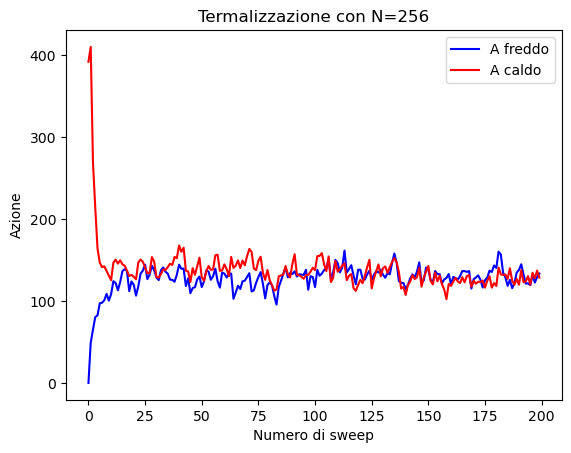
\includegraphics[width=0.8\textwidth]{images/thermalisation_N256.png}
    \caption{Termalizzazione per $N=256$ e $\Delta=1$.}
    \label{grafico termalizzazione}
\end{figure}

In Figura \ref{grafico termalizzazione} osserviamo come dopo 200 sweep si è ampiamente raggiunta la termalizzazione, sia partendo da caldo che da freddo. Questo comportamento si osserva anche per gli altri valori di $N$. Possiamo pertanto porre il tempo di termalizzazione
\begin{equation}
    \label{tempo termalizzazione}
    \tau_{\textup{term}}\simeq 200, 
\end{equation}
e quindi saltare i primi 200 sweep nella simulazione effettiva. 

\subsubsection{Dipendenza da $\Delta$}
Il tempo di termalizzazione dipende da quanto la catena evolve velocemente. Se $\Delta$ è molto piccolo, i valori proposti dal Metropolis sono molto vicini a quelli precedenti, pertanto l'azione varierà poco quando si effettua uno sweep e ci aspettiamo un aumento del tempo di termalizzazione, nonostante avremo un'accettanza molto alta. In Figura \ref{grafico mancata termalizzazione} osserviamo come con $\Delta=0.1$ e $N=256$, 200 sweep non sono sufficienti a raggiungere la termalizzazione (al contrario del caso in Figura \ref{grafico termalizzazione}), in quanto abbiamo una catena che evolve molto lentamente.
\begin{figure}[h]
    \centering
    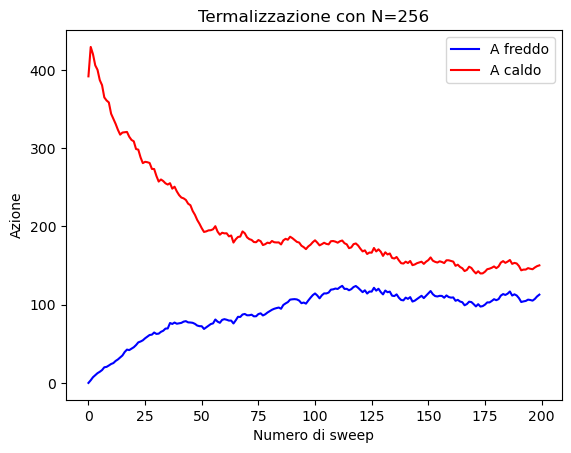
\includegraphics[width=0.8\textwidth]{images/thermalisation_N256_Delta01.png}
    \caption{Dopo 200 sweep, con $\Delta=0.1$ e $N=256$ non si è ancora raggiunta la termalizzazione a causa di una evoluzione molto lenta della catena.}
    \label{grafico mancata termalizzazione}
\end{figure}


\subsection{Tempo di autocorrelazione}

Per valutare il tempo di autocorrelazione, necessario per stabiliare la grandezza dei bin, possiamo calcolare la funzione $\Gamma$ definita in (\ref{equazione gamma}), che abbiamo visto quantifica la deviazione dal caso di variabili scorrelate. Si osserva che tale funzione ha un andamento esponenziale nel tempo markoviano, possiamo quindi stimare il tempo di autocorrelazione a partire dalla costante di decadimento di tale esponenziale. Tramite un fit esponenziale su $\Gamma$ ricaviamo i tempi di decadimento, che sono riportati in Tabella \ref{tabella autocorrelazione}.
\begin{table}[h]
    \centering
    \begin{tabular}{||c c c c c c c||} 
     \hline
     $t$ & $N=32$ & $N=64$ & $N=128$ & $N=256$ & $N=512$ & $N=1024$ \\ [0.5ex] 
     \hline\hline
     1 & 2.18 & 4.38 & 9.50 & 23.3 & 78.2 & 387\\
     2 & 2.01 & 3.98 & 9.86 & 24.5 & 81.0 & 395\\
     3 & 1.99 & 3.73 & 9.68 & 25.5 & 84.2 & 405\\
     4 & 2.00 & 3.67 & 9.30 & 26.0 & 87.1 & 417\\
     5 & 1.98 & 3.67 & 9.00 & 25.9 & 89.3 & 428\\[1ex] 
     \hline
    \end{tabular}
    \caption{Tempi di decadimento di $\Gamma$ al variare di $t$ per vari passi reticolari. Riportiamo a titolo di esempio solo i primi valori di $t$.}
    \label{tabella autocorrelazione}
\end{table}

Riportiamo come esempio in Figura \ref{grafico gamma non binnata} la rappresentazione in scala logaritmica di $\frac{\Gamma(t_M)}{\Gamma(0)}$, calcolata per $N=128$ e $t=2$. 
\begin{figure}[h]
    \centering
    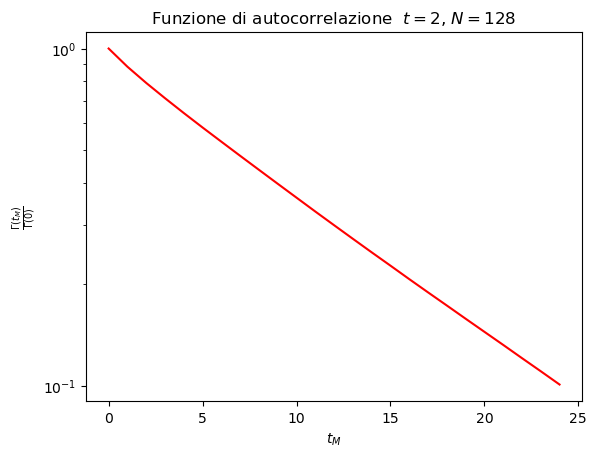
\includegraphics[width=0.8\textwidth]{images/gamma_t2_N128.png}
    \caption{Funzione di autocorrelazione, in scala logaritmica, calcolata per $t=2$ e $N=128$, con 1350000 sweep.}
    \label{grafico gamma non binnata}
\end{figure}

A partire dai tempi di decadimento della Tabella \ref{tabella autocorrelazione} possiamo stabilire la grandezza dei bin prendendo circa 10 volte il tempo di autocorrelazione medio. Come si osserva il tempo di decadimento dipende sensibilmente dal passo reticolare, conseguentemente passi reticolari più piccoli avranno bin di dimensione maggiore. Questo porta ad avere una simulazione sempre più costosa per passi reticolari più piccoli a parità di dati binnati, siccome i bin hanno dimensione maggiore (oltre al fatto che essendo $N$ maggiore andranno processati più dati a ogni sweep). Riportiamo le grandezze dei bin scelte in Tabella \ref{tabella D_BIN}. 
\begin{table}[h]
    \centering
    \begin{tabular}{||c||c c c c c c||} 
     \hline
     $N$ & 32 & 64& 128 & 256 & 512 &1024 \\
     $D_{\textup{BIN}}$ & 20 & 40 & 90 & 250 & 800 &2500 \\[1ex] 
     \hline
    \end{tabular}
    \caption{Dimensione dei bin al variare del passo reticolare.}
    \label{tabella D_BIN}
\end{table}

Vogliamo inoltre verificare che una volta effettuato il binnaggio i correlatori descritti nell'equazione (\ref{cbinnate}) risultano essere scorrelati tra loro a tempi markoviani diversi.
A tal scopo possiamo effettuare il binnaggio e ricalcolare la funzione $\Gamma$ dopo il binnaggio. Ci aspettiamo che ora la funzione di autocorrelazione decada molto velocemente a zero. Riportiamo il risultato per $N=128$ e $t=2$ nella Figura \ref{grafico gamma binnata}, affiancato a quello precedente in scala lineare.
\begin{figure}[h]
    \centering
    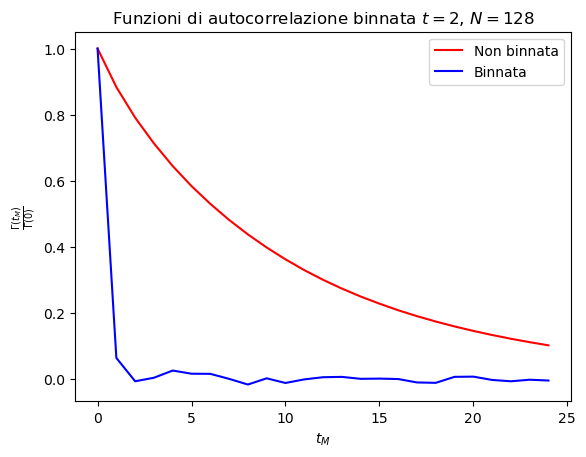
\includegraphics[width=0.8\textwidth]{images/gammabinnata_t2_N128.png}
    \caption{Funzioni di autocorrelazione prima e dopo il binnaggio, calcolate per $t=2$ e $N=128$, con 1350000 sweep.}
    \label{grafico gamma binnata}
\end{figure}

Il comportamento osservato conferma il fatto che i correlatori binnati possono essere considerati come estrazioni indipendenti.

\subsubsection{Dipendenza da $\Delta$}
Abbiamo visto precedentemente come variare $\Delta$ varia la velocità di evoluzione della catena. Ci aspettiamo pertanto che il valore di $\Delta$ influenzi anche il tempo di autocorrelazione, in particolare:
\begin{itemize}
    \item un valore basso di $\Delta$ porta a una catena che si muove lentamente e quindi a un tempo di autocorrelazione più alto;
    \item un valore alto di $\Delta$ porta a una catena che evolve più velocemente e quindi un tempo di autocorrelazione più basso.
\end{itemize}
In Figura \ref{grafico gamma varie delta} è rappresentata la funzione di autocorrelazione per vari valori di $\Delta$, nella quale osserviamo il comportamento descritto. 
\begin{figure}[h]
    \centering
    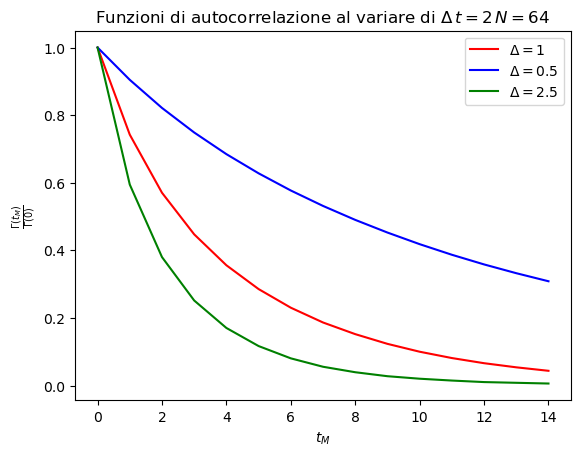
\includegraphics[width=0.8\textwidth]{images/gamma_differentDelta.png}
    \caption{Funzioni di autocorrelazione, calcolate per $t=2$ e $N=64$, a vari valori di $\Delta$.}
    \label{grafico gamma varie delta}
\end{figure}

Una scelta corretta di $\Delta$ pertanto punta ad avere dei bin di lunghezza minore, che si traduce in una simulazione più efficiente. 



\subsection{Calcolo dell'energia}
Riassumendo i parametri scelti per il calcolo del correlatore risultano:
\begin{itemize}
    \item $\Delta=1$;
    \item tempo di termalizzazione pari a 200 step;
    \item dimensione dei bin e numero di bin in Tabella \ref{durata simulazione}.
\end{itemize}
\begin{table}[h]
    \centering
    \begin{tabular}{||c c c||} 
     \hline
     $N$ & $D_{\textup{BIN}}$ & $N_{\textup{BIN}}$\\ [0.5ex] 
     \hline\hline
     32 & 20 & 5 milioni\\
     64 & 40 & 2.5 milioni\\
     128 & 90 & 1 milione\\
     256 & 250 & 500 mila\\
     512 & 800 & 50 mila\\
     1024 & 2500 & 10 mila\\[1ex] 
     \hline
    \end{tabular}
    \caption{Dimensione e numero dei bin al variare del passo reticolare.}
    \label{durata simulazione}
\end{table}

Mentre sulla dimensione dei bin abbiamo dei vincoli dati dal tempo di autocorrelazione, per quanto riguarda il numero di bin la scelta è a nostra discrezione. Ovviamente avere un numero di bin maggiore porta a una stima migliore dell'osservabile, però al crescere di $N$ l'aumentare della dimensione dei bin e del numero di variabili di integrazione da estrarre con il Metropolis porta ad avere un calcolo sempre più lungo. Pertanto la scelta va fatta anche in modo da avere una simulazione di durata contenuta. In Tabella \ref{pollo allo spiedo} sono riportati i tempi riscontrati con i valori scelti.
\begin{table}[h]
    \centering
    \begin{tabular}{||c c ||} 
     \hline
     $N$ & Durata simulazione (minuti)\\ [0.5ex] 
     \hline\hline
     32 & 24\\
     64 & 32\\
     128 &53\\
     256 &215\\
     512 &200\\
     1024 &418\\[1ex] 
     \hline
    \end{tabular}
    \caption{Dimensione e numero dei bin al variare del passo reticolare.}
    \label{pollo allo spiedo}
\end{table}

Il calcolo dell'energia tramite l'equazione (\ref{nuvola}) viene effettuato per ogni set di parametri in Tabella \ref{durata simulazione} e per ogni valore di $t$. Andiamo poi a scartare i valori di $t$ che presentano un errore relativo superiore al 10\% e mediamo sui restanti, come descritto nella sezione 2.8, propagando l'errore utilizzando il Jackknife. Riportiamo in Tabella \ref{tabella energie simulate} i risultati ottenuti di energia, con il relativo errore, assieme ai risultati esatti su reticolo, che possono essere calcolati a partire dell'equazione (\ref{energia esatto}). È riportato inoltre un test di compatibilità tra i due valori, calcolato prendendo $\frac{|\textup{valore stimato - valore atteso}|}{\textup{errore valore stimato}}$.
\begin{table}[h]
    \centering
    \begin{tabular}{||c c c c||} 
     \hline
     $a$ & valore esatto & valore calcolato & compatibilità\\[0.5ex] 
     \hline\hline
     2      & 0.88137  & 0.88137  $\pm$ 0.00018 & 0.9 \\
     1      & 0.96242  & 0.96221 $\pm$ 0.00017 & 1.3 \\
     0.5    & 0.98986  & 0.98989 $\pm$ 0.00021 & 0.1 \\
     0.25   & 0.99741  & 0.99726  $\pm$ 0.00026 & 0.5 \\
     0.125  & 0.9993  & 0.9986 $\pm$ 0.0008 & 0.9 \\
     0.0625 & 0.9998  & 1.0010 $\pm$ 0.0019 & 0.6 \\[1ex] 
     \hline
    \end{tabular}
    \caption{Valore esatto e valore calcolato dell'energy gap $\varepsilon_1-\varepsilon_0$ al variare del passo reticolare.}
    \label{tabella energie simulate}
\end{table}\\
Per ottenere il valore dell'energy gap nel continuo è necessario affidarsi all'equazione (\ref{eps=E+o(a)}) ed effettuare una estrapolazione ad $a=0$. In particolare sappiamo che 
\begin{equation}
    \varepsilon_1-\varepsilon_0=E_1-E_0+\sum_{n=0}^{+\infty}\alpha_{2n}\,a^{2n}.
\end{equation}
L'estrapolazione viene effettuata tramite un fit polinomiale, il cui termine noto ci fornirà il valore $E_1-E_0$ cercato nel continuo. È possibile effettuare un fit lineare in $a^2$, oppure quadratico in $a^2$. Per una maggiore precisione usiamo il secondo, quindi effettuiamo il fit con la funzione 
\begin{equation}
    f(a^2)=\alpha+\beta a^2+\gamma a^4.
\end{equation}
Il termine noto $\alpha$ sarà una stima di $E_1-E_0$.
Con un polinomio di ordine così basso tuttavia il punto in $a=2$ ($N=32$) risulta troppo lontano dall'origine per poter rientrare nel fit. Includerlo infatti porta a risultati imprecisi. Per utilizzarlo sarebbe necessario utilizzare un fit con termini di ordine più alto, ma ciò comporterebbe introdurre più parametri di fit; per semplicità è preferibile mantenere il fit quadratico in $a^2$. Scartiamo quindi il punto in questione ed effettuiamo il fit. 
In Figura \ref{grafico estrapolazione deltaE} e in Tabella \ref{tabella energie continuo} sono riportati i risultati, assieme a un test di compatibilità con il valore esatto nel continuo. 
\begin{figure}[h]
    \centering
    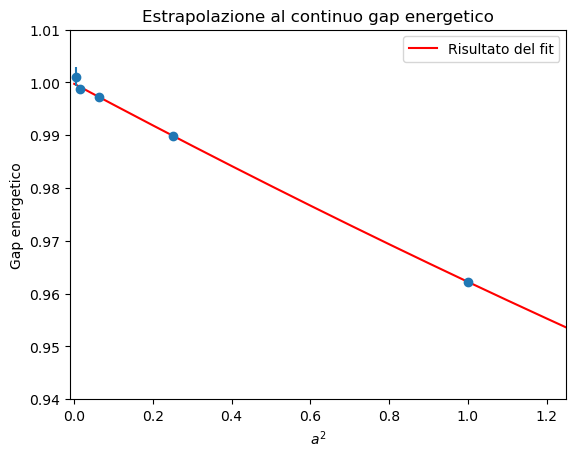
\includegraphics[width=0.8\textwidth]{images/deltaE_estrapolazione.png}
    \caption{Estrapolazione al continuo dell'energy gap $E_1-E_0$.}
    \label{grafico estrapolazione deltaE}
\end{figure}
\begin{table}[h]
    \centering
    \begin{tabular}{||c c c c||} 
     \hline
    $\Delta E$ esatto & $\Delta E$ stimato & $\chi^2$ ridotto & compatibilità\\[0.5ex] 
     \hline\hline
     1 & 0.99971 $\pm$ 0.00034 & 0.5 & 0.8 \\[1ex] 
     \hline
    \end{tabular}
    \caption{Valore esatto e valore calcolato dell'energy gap $E_1-E_0$ nel continuo.}
    \label{tabella energie continuo}
\end{table}

Siccome in questo caso è nota l'espressione esatta dell'andamento a passo reticolare finito (eq. (\ref{energia esatto})), possiamo approfondire l'analisi effettuata nella scelta del polinomio interpolante. In particolare a partire dalla (\ref{energia esatto}), con i valori scelti di $\omega=1$ e $m=1$ si trova che 
\begin{equation}
    \label{espansione errore energia}
    \varepsilon_1-\varepsilon_0=1-\frac{1}{24}a^2+\frac{3}{640}a^4+O(a^6).
\end{equation}
In Figura \ref{grafico quadratico quartico} è rappresentato l'andamento esatto confrontato con la sua approssimazione lineare e quadratica in $a^2$. Come si osserva il punto in $a=2$ non è ben approssimato dall'approssimazione quadratica, pertanto per evitare di considerare potenze superiore è necessario scartarlo. I restanti punti invece risultano in linea con l'approssimazione quadratica.
\begin{figure}[h]
    \centering
    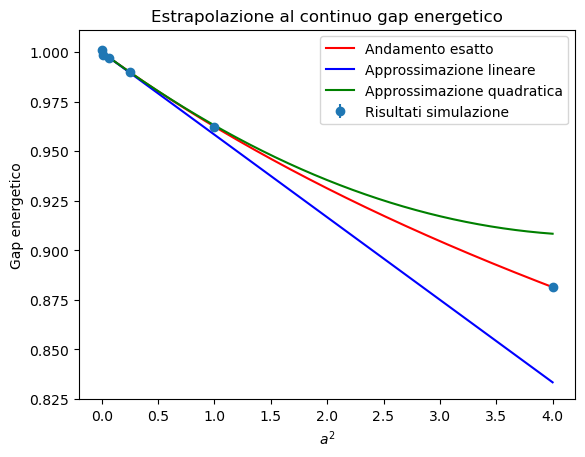
\includegraphics[width=0.8\textwidth]{images/deltaE_esatto_vs_quad_vs_quart.png}
    \caption{Confronto tra $\Delta\varepsilon(a)$ esatto e la sua approssimazione lineare e quadratica in $a^2$.}
    \label{grafico quadratico quartico}
\end{figure}


\subsection{Calcolo dell'elemento di matrice}
Per l'elemento di matrice si segue la stessa procedura utilizzata per l'energy gap. Riportiamo in Tabella \ref{tabella matrix simulate} i risultati ottenuti dalla simulazione a passo reticolare finito, con il relativo errore, assieme ai risultati esatti, calcolati a partire dell'equazione (\ref{el mat esatto}).
\begin{table}[h]
    \centering
    \begin{tabular}{||c c c c||} 
     \hline
     $a$ & valore esatto & valore calcolato & compatibilità\\[0.5ex] 
     \hline\hline
     2      & 0.88137  & 0.59454  $\pm$ 0.00003 & 2.2 \\
     1      & 0.96242  & 0.66871 $\pm$ 0.00004 & 0.8 \\
     0.5    & 0.98986  & 0.69646 $\pm$ 0.00004 & 0.2 \\
     0.25   & 0.99741  & 0.70430  $\pm$ 0.00005 & 1.3 \\
     0.125  & 0.9993  & 0.70620 $\pm$ 0.00015 & 1.4 \\
     0.0625 & 0.9998  & 0.7067 $\pm$ 0.0004 & 0.8 \\[1ex] 
     \hline
    \end{tabular}
    \caption{Valore esatto e valore calcolato dell'elemento di matrice $\left<\varepsilon_0\right|\hat{x}\left|\varepsilon_1\right>$ al variare del passo reticolare.}
    \label{tabella matrix simulate}
\end{table}

Possiamo anche qua scartare il punto con $a=2$ per evitare di considerare potenze troppo alte. Usiamo quindi ancora come funzione di fit
\begin{equation}
    f(a^2)=\alpha+\beta a^2+\gamma a^4,
\end{equation}
con il termine noto che sarà il valore cercato nel continuo. In Figura \ref{grafico estrapolazione matrice} e in Tabella \ref{tabella energie matrice} sono riportati i risultati del fit.
\begin{figure}[h]
    \centering
    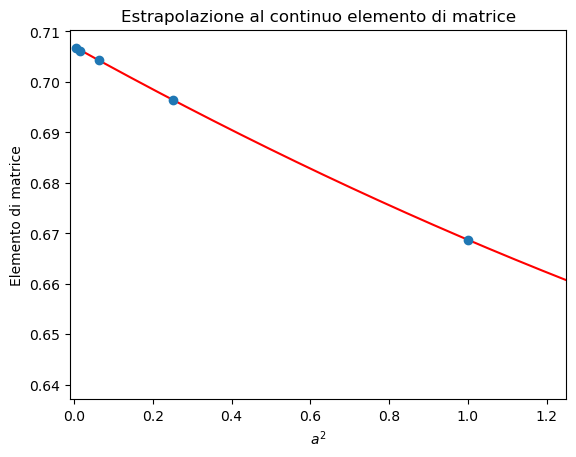
\includegraphics[width=0.8\textwidth]{images/matrix_el_estrapolazione.png}
    \caption{Estrapolazione al continuo dell'elemento di matrice $\left<0\right|\hat{x}\left|1\right>$.}
    \label{grafico estrapolazione matrice}
\end{figure}
\begin{table}[h]
    \centering
    \begin{tabular}{||c c c c||} 
     \hline
    $\left<0\right|\hat{x}\left|1\right>$ esatto & $\left<0\right|\hat{x}\left|1\right>$ stimato & $\chi^2$ ridotto & compatibilità\\[0.5ex] 
     \hline\hline
     0.70711 & 0.70697$\pm$ 0.00007 & 0.3 & 2\\[1ex] 
     \hline
    \end{tabular}
    \caption{Valore esatto e valore calcolato dell'elemento di matrice $\left<0\right|\hat{x}\left|1\right>$ nel continuo.}
    \label{tabella energie matrice}
\end{table}

Anche in questo caso analizziamo la scelta del polinomio interpolante. Espandendo l'equazione (\ref{el mat esatto}) troviamo che, per i valori $\omega=1$ e $m=1$
\begin{equation}
    \left<\varepsilon_0\right|\hat{x}\left|\varepsilon_1\right>=\frac{1}{\sqrt{2}}-\frac{1}{16\sqrt{2}}\,a^2+\frac{5}{512\sqrt{2}}\,a^4+O(a^6).
\end{equation}
In Figura \ref{grafico quadratico quartico matrice} è riportato come prima l'andamento esatto e l'approssimazione troncata al primo e secondo ordine in $a^2$.
\begin{figure}[h]
    \centering
    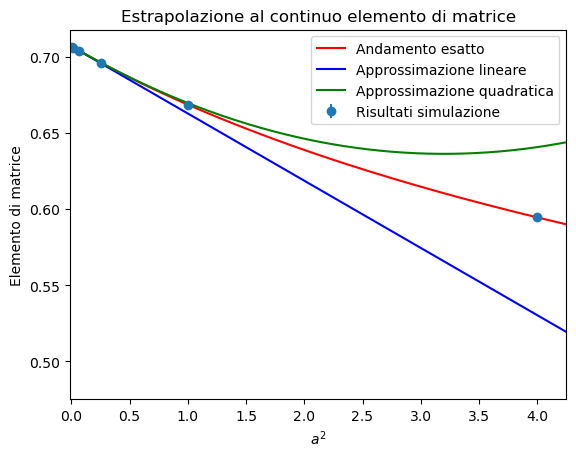
\includegraphics[width=0.8\textwidth]{images/matrixel_esatto_vs_quad_vs_quart.png}
    \caption{Confronto tra $\left<\varepsilon_0\right|\hat{x}\left|\varepsilon_1\right>(a)$ esatto e la sua approssimazione lineare e quadratica.}
    \label{grafico quadratico quartico matrice}
\end{figure}

Anche in questo caso si osserva che il punto in $a=2$ non è ben descritto da una approssimazione in potenze così basse, mentre i restanti punti risultano in linea come ci attendevamo.

\section{Conclusioni}
Abbiamo calcolato l'energy gap $E_1-E_0$ tra i primi due livelli di un oscillatore armonico con $\omega=1$ e $m=1$, e l'elemento di matrice $\left<0\right|\hat{x}\left|1\right>$, ottenendo come risultato finale 
$$E_1-E_0=0.99971 \pm 0.00034,$$
$$\left<0\right|\hat{x}\left|1\right>=0.70697\pm 0.00007,$$
con un errore relativo dell'ordine di $10^{-4}$.\\
 La tecnica utilizzata consiste nel calcolare la funzione di correlazione a due punti mediante un metodo Montecarlo che estrae numeri con l'algoritmo del Metropolis. A partire dal correlatore è poi possibile estrarre varie quantità fisiche. L'importanza del metodo illustrato risiede nel fatto che può essere applicato per calcolare quantità più complesse, e con le dovute generalizzazioni anche in teoria quantistica dei campi.







\end{document}
